\chapter{Design of Steel Sheet Pile}
%\label{appendix:structural}

\section{Vertical effective stress}

\begin{table}[H]
  \centering
  \caption{Vertical effective stress on left and right sides}
  \label{tab:appendix_effective_stress}
  \small
  \setlength{\tabcolsep}{8pt}
  \renewcommand{\arraystretch}{1.15}
  \begin{tabular}{@{}r r r@{}}
    \toprule
    $z$ [m] &
    $\sigma'_{z,l}$ [kN/m$^2$] &
    $\sigma'_{z,r}$ [kN/m$^2$] \\
    \midrule
     0.00 &  0.00 &  0.00 \\
     1.47 &  0.00 & 17.64 \\
     2.00 &  0.00 & 18.80 \\
     4.00 &  0.00 & 37.18 \\
     7.00 & 27.57 & 64.75 \\
    10.00 & 40.14 & 77.32 \\
    \bottomrule
  \end{tabular}
\end{table}

\section{Earth pressure and force}
\label{appendix:earth_pressure}

\subsection{Earth pressure}

\begin{figure}[H]
    \centering
    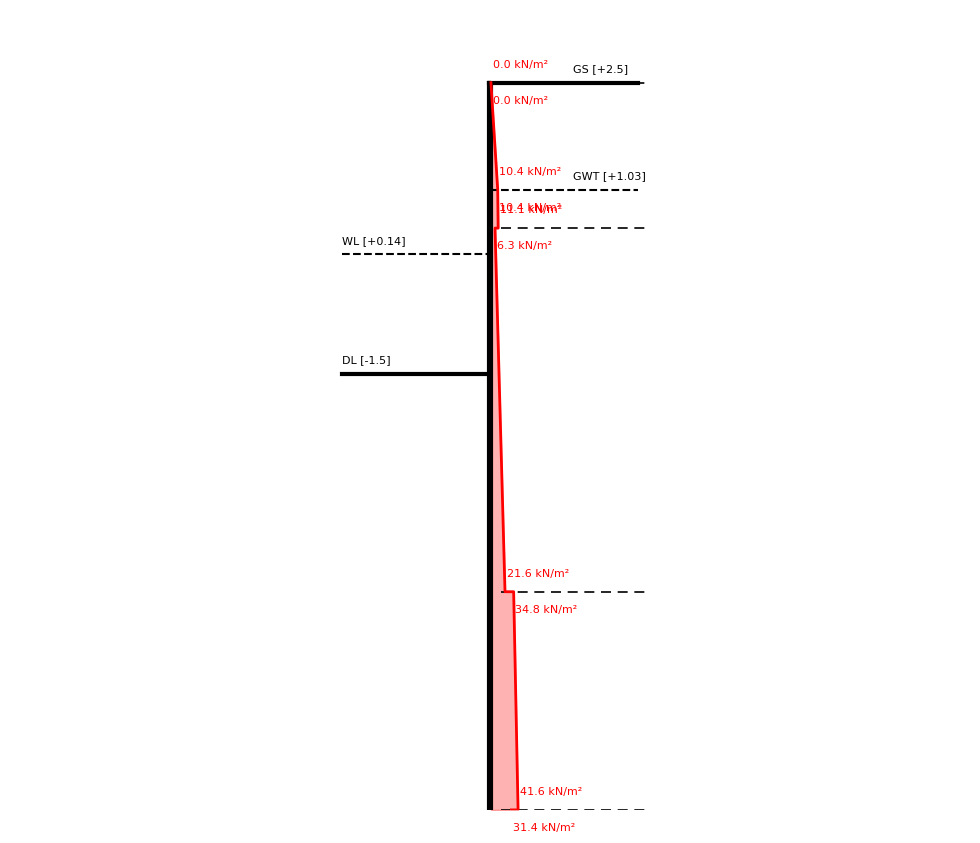
\includegraphics[width=0.75\linewidth]{figures/appendix-i/active_earth_pressure.png}
    \caption{"ACTIVE" earth pressures}
    \label{fig:appendix_earth_pressure}
\end{figure}

\begin{table}[H]
  \centering
  \caption{"ACTIVE" earth pressure coefficients and pressures}
  \label{tab:appendix_active_pressures}
  \small
  \setlength{\tabcolsep}{8pt}
  \renewcommand{\arraystretch}{1.15}
  \begin{tabular}{@{}r r r r r@{}}
    \toprule
    $z$ [m] &
    $K_{a,\text{above}}$ &
    $K_{a,\text{below}}$ &
    $p_{\text{above}}$ [kN/m$^2$] &
    $p_{\text{below}}$ [kN/m$^2$] \\
    \midrule
     0.00 & 0.589 & 0.589 &  0.00 &  0.00 \\
     1.47 & 0.589 & 0.589 & 10.39 & 10.39 \\
     2.00 & 0.589 & 0.333 & 11.07 &  6.27 \\
     7.00 & 0.333 & 0.538 & 21.58 & 34.81 \\
    10.00 & 0.538 & 0.406 & 41.57 & 31.38 \\
    \bottomrule
  \end{tabular}
\end{table}

\begin{figure}[H]
    \centering
    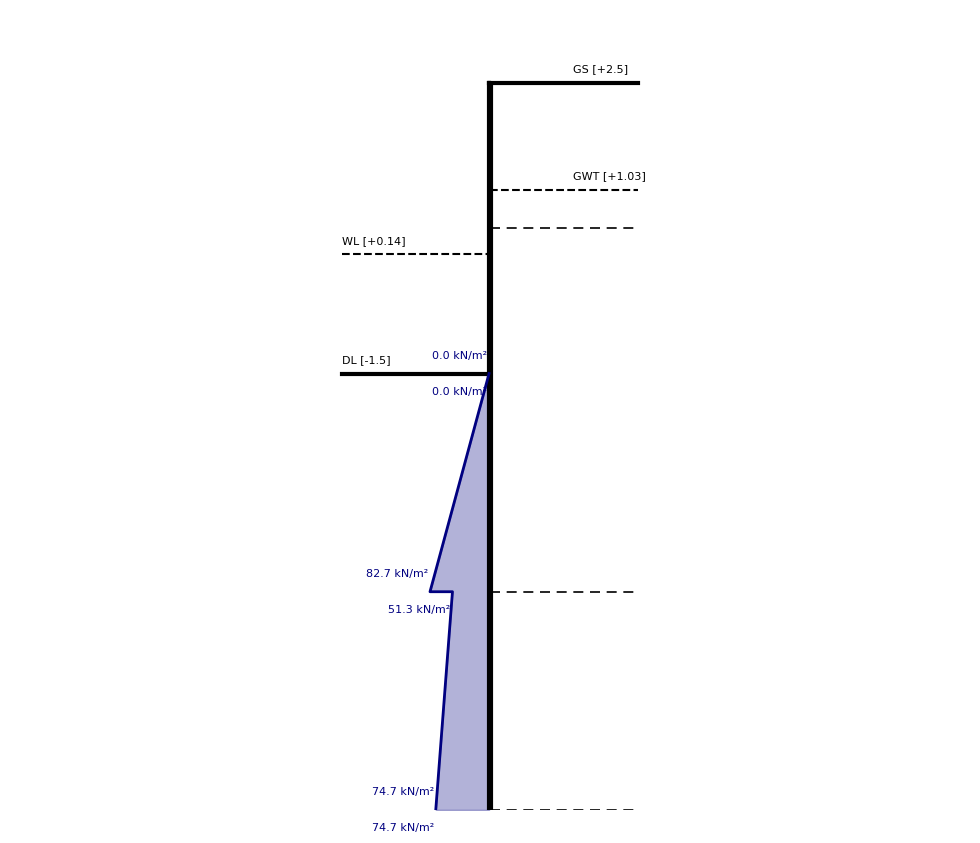
\includegraphics[width=0.75\linewidth]{figures/appendix-i/passive_earth_pressure.png}
    \caption{"PASSIVE" earth pressures}
    \label{fig:appendix_passive_earth_pressure}
\end{figure}

\begin{table}[H]
  \centering
  \caption{"PASSIVE" earth pressure coefficients and pressures}
  \label{tab:appendix_passive_pressures_coeffiecients}
  \small
  \setlength{\tabcolsep}{8pt}
  \renewcommand{\arraystretch}{1.15}
  \begin{tabular}{@{}r r r r r@{}}
    \toprule
    $z$ [m] &
    $K_{p,\text{above}}$ &
    $K_{p,\text{below}}$ &
    $p_{\text{above}}$ [kN/m$^2$] &
    $p_{\text{below}}$ [kN/m$^2$] \\
    \midrule
     4.00 & 3.000 & 3.000 &  0.00 &  0.00 \\
     7.00 & 3.000 & 1.860 & 82.71 & 51.28 \\
    10.00 & 1.860 & 1.860 & 74.66 & 74.66 \\
    \bottomrule
  \end{tabular}
\end{table}

\subsection{Forces}

\begin{table}[H]
  \centering
  \caption{Resultant forces and centroids by segment}
  \label{tab:appendix_forces_centroids}
  \small
  \setlength{\tabcolsep}{8pt}
  \renewcommand{\arraystretch}{1.15}
  \begin{tabular}{@{}l r l r r@{}}
    \toprule
    Side & Segment & Shape &
    F [kN/m] & $z_c$ [m] \\
    \midrule
    "ACTIVE" & 1 & Triangle  &  7.63 & 0.98 \\
    "ACTIVE" & 2 & Rectangle &  5.50 & 1.73 \\
    "ACTIVE" & 2 & Triangle  &  0.18 & 1.82 \\
    "ACTIVE" & 3 & Rectangle & 31.33 & 4.50 \\
    "ACTIVE" & 3 & Triangle  & 38.29 & 5.33 \\
    "ACTIVE" & 4 & Rectangle & 104.44 & 8.50 \\
    "ACTIVE" & 4 & Triangle  & 10.14 & 9.00 \\
    "PASSIVE" & 1 & Triangle  & 124.06 & 6.00 \\
    "PASSIVE" & 2 & Rectangle & 153.84 & 8.50 \\
    "PASSIVE" & 2 & Triangle  &  35.07 & 9.00 \\
    \bottomrule
  \end{tabular}
\end{table}

\section{Hydrostatic pressure and force}

\begin{table}[H]
  \centering
  \caption{Pore pressure values along depth}
  \label{tab:appenidx_u_profile}
  \small
  \setlength{\tabcolsep}{8pt}
  \renewcommand{\arraystretch}{1.15}
  \begin{tabular}{@{}l l l l@{}}
    \toprule
    \textbf{$z$ [m]} &
    \textbf{$u_{right}$ [kN/m$^2$]} &
    \textbf{$u_{left}$ [kN/m$^2$]} &
    \textbf{$u_{net}$ [kN/m$^2$]} \\
    \midrule
     0.00  &  0.00  &  0.00  &  0.00 \\
     1.47  &  0.00  &  0.00  &  0.00 \\
     2.00  &  5.20  &  0.00  &  5.20 \\
     2.36  &  8.73  &  0.00  &  8.73 \\
     7.00  & 54.25  & 45.52  &  8.73 \\
    10.00  & 83.68  & 74.95  &  8.73 \\
    \bottomrule
  \end{tabular}
\end{table}

\section{Bending moment}

\begin{figure}[H]
    \centering
    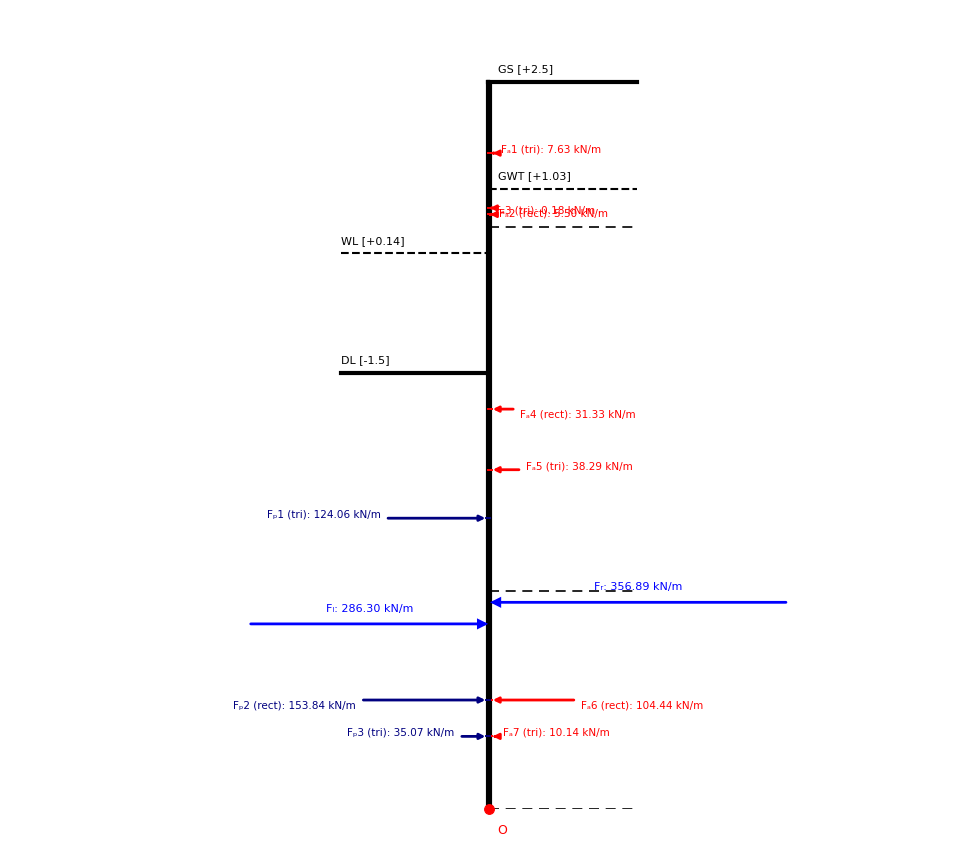
\includegraphics[width=0.90\linewidth]{figures/appendix-i/point_O_forces_combined.png}
    \caption{Forces for $t = 6.00$ meters}
    \label{fig:appendix_moments_balance_6000}
\end{figure}

\begin{table}[H]
  \centering
  \caption{Resultant forces, arms, and moments for $t = 6.0$ meters}
  \label{tab:appendix_forces_arms_moments_now}
  \small
  \setlength{\tabcolsep}{8pt}
  \renewcommand{\arraystretch}{1.15}
  \begin{tabular}{@{}l l r r r@{}}
    \toprule
    Side & Shape &
    F [kN/m] & $z_{base}$[m] &
    $M_{\text{base}}$ [kN$\cdot$m/m] \\
    \midrule
    ACTIVE & Triangle  &  7.63  & 9.02 &  68.86 \\
    ACTIVE & Rectangle &  5.50  & 8.27 &  45.50 \\
    ACTIVE & Triangle  &  0.18  & 8.18 &   1.48 \\
    ACTIVE & Rectangle & 31.33  & 5.50 & 172.34 \\
    ACTIVE & Triangle  & 38.29  & 4.67 & 178.69 \\
    ACTIVE & Rectangle & 104.44  & 1.50 & 156.65 \\
    ACTIVE & Triangle  & 10.14  & 1.00 &  10.14 \\
    HYDRO PASSIVE & Triangle  & 286.30  & 2.55 &  -730.07 \\
    HYDRO ACTIVE & Triangle  & 356.89  & 2.84 &  1014.8 \\
    PASSIVE & Triangle  & 124.06 & 4.00 & -496.26 \\
    PASSIVE & Rectangle & 153.84 & 1.50 & -230.76 \\
    PASSIVE & Triangle  &  35.07 & 1.00 &  -35.07 \\
    \midrule
    $\sum{M_{t}}$ (should ≈ 0 for equilibrium) &  &  & & 156.3 \\
    \bottomrule
  \end{tabular}
\end{table}

\section{Ultimate Limit and Serviceability Limit State}
\label{appendix:uls_combinations}

\subsection{DA1-1}

\begin{table}[H]
  \centering
  \caption{Design values soil DA1-1}
  \label{tab:soil_layers_DA1_1}
  \small
  \setlength{\tabcolsep}{6pt}
  \renewcommand{\arraystretch}{1.15}
  \begin{tabularx}{\linewidth}{@{}p{1.6cm}l p{1.6cm}*{5}{Y}@{}}
    \toprule
    Layer &
    Soil type &
    Depth [m] &
    $\gamma_d\,[\mathrm{kN/m}^3]$ &
    $\gamma_{\!sat}\,[\mathrm{kN/m}^3]$ &
    $\varphi'\,[{}^\circ]$ &
    ${c'}\,[\mathrm{kPa}]$ &
    ${c_u}\,[\mathrm{kPa}]$ \\
    \midrule
    1 & Fill               & 0.0 - 2.0   & 12 & 12 & 15.0 & 2.5 & 20 \\
    2 & Fine/medium sand   & 2.0 - 7.0   & 17 & 19 & 30.0 & 0.0 & \textemdash \\
    3 & Clay               & 7.0 - 10.0  & 14 & 14 & 17.5 & 0.0 & 25 \\
    4 & Clayey sand        & 10.0 - 15.0 & 18 & 20 & 25.0 & 0.0 & \textemdash \\
    5 & Clay               & 15.0 - 16.0 & 14 & 14 & 17.5 & 0.0 & 25 \\
    6 & Clayey sand        & 16.0 - 17.5 & 18 & 20 & 25.0 & 0.0 & \textemdash \\
    7 & Medium sand        & 17.5 - 32.0 & 18 & 20 & 32.5 & 0.0 & \textemdash \\
    \bottomrule
  \end{tabularx}
\end{table}

\begin{figure}[H]
    \centering
    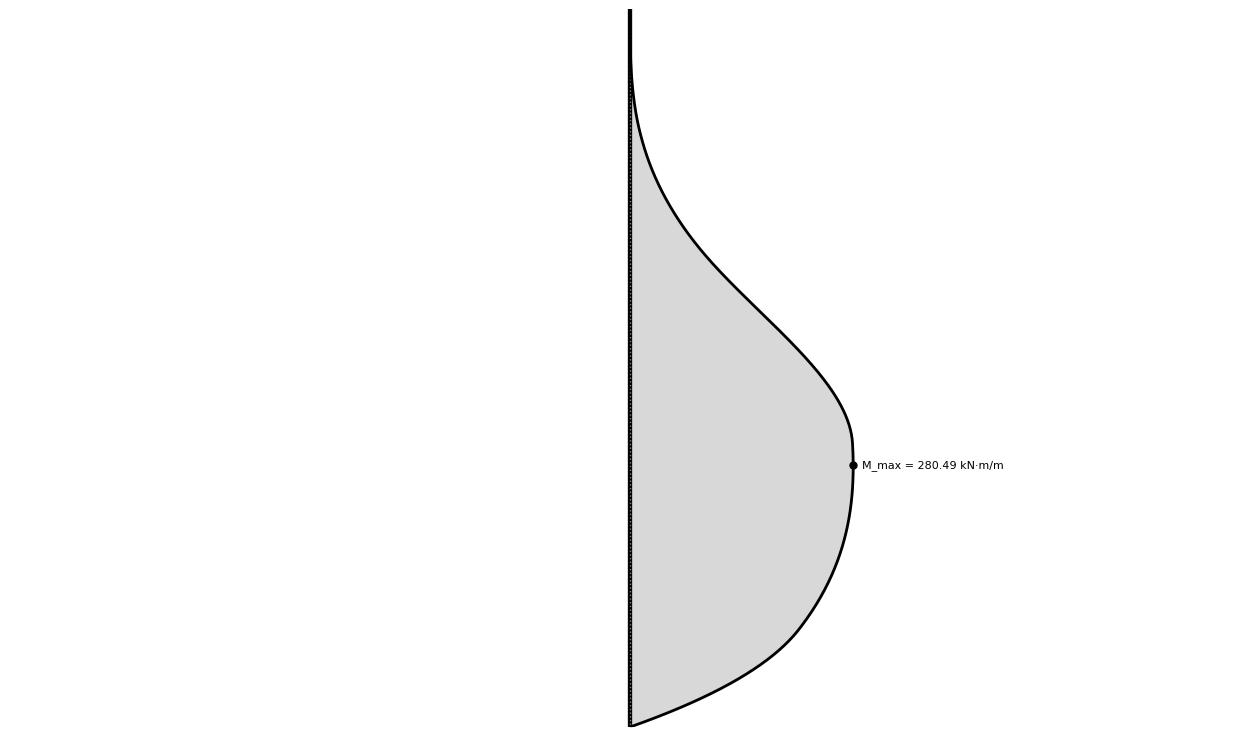
\includegraphics[width=0.80\linewidth]{figures/appendix-i/bending_moments_line_DA1_1.png}
    \caption{Bending moment line DA1-1}
    \label{fig:appendix_bending_moments_DA1_1}
\end{figure}

\begin{table}[H]
  \centering
  \caption{Moment calculation summary DA1-1}
  \label{tab:moment_summary}
  \small
  \setlength{\tabcolsep}{8pt}
  \renewcommand{\arraystretch}{1.15}
  \begin{tabular}{@{}l r@{}}
    \toprule
    Quantity & Value \\
    \midrule
    Depth below ground [m] & 7.374 \\
    Depth below dredge [m] & 3.374 \\
    $M_{a,\text{soil}}(S)$ [kN·m/m] & 339.481 \\
    $M_{wR}(S)$ [kN·m/m] & 454.148 \\
    $M_{a}(S) = M_{a,\text{soil}} + M_{wR}$ [kN·m/m] & 793.629 \\
    $M_{p,\text{soil}}(S)$ [kN·m/m] & 234.980 \\
    $M_{wL}(S)$ [kN·m/m] & 278.160 \\
    $M_{p}(S) = M_{p,\text{soil}} + M_{wL}$ [kN·m/m] & 513.140 \\
    $M_{\text{max}} = M_{a}(S) - M_{p}(S)$ [kN·m/m] & 280.489 \\
    \bottomrule
  \end{tabular}
\end{table}

\begin{figure}[H]
    \centering
    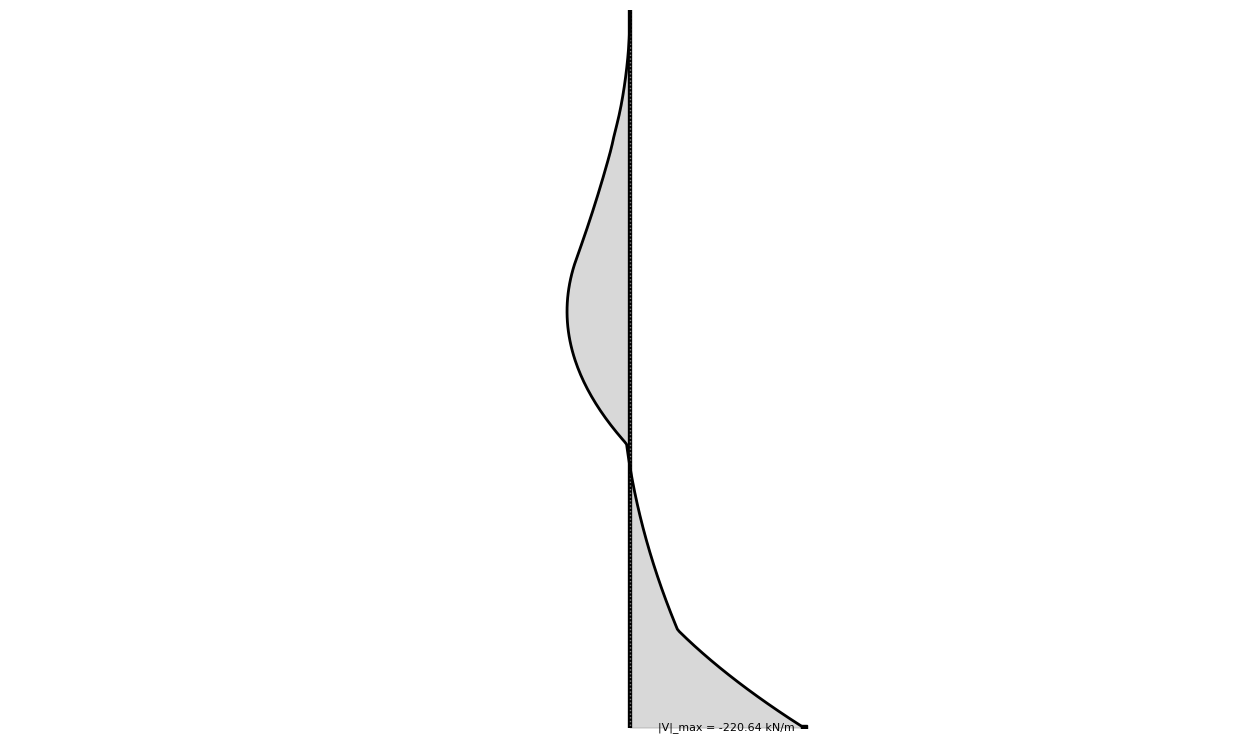
\includegraphics[width=0.80\linewidth]{figures/appendix-i/shear_line_7575.png}
    \caption{Shear force line DA1-1}
    \label{fig:appendix_shear_forces_DA1_1}
\end{figure}

\begin{table}[H]
  \centering
  \caption{Shear and partial-resultants summary}
  \label{tab:shear_summary_zs}
  \small
  \setlength{\tabcolsep}{10pt}
  \renewcommand{\arraystretch}{1.15}
  \begin{tabular}{@{}l r@{}}
    \toprule
    Quantity & Value \\
    \midrule
    Zero-shear depth $z_S$ [m] & 7.374 \\
    Depth below dredge at $z_S$ [m] & 3.374 \\
    $V(0)$ at ground [kN/m] & 0.000 \\
    $V(Z)$ at dredge [kN/m] & 67.749 \\
    $V(z_S)$ [kN/m] & -0.000 \\
    $V(z_{\text{toe}})$ [kN/m] & -220.641 \\
    $|V|_{\max}$ [kN/m] & -220.641 \\
    Depth of $|V|_{\max}$ [m] & 11.575 \\
    $V_a(0\to z_S)$ [kN/m] & 129.746 \\
    $V_{wR}(\text{wt}\to z_S)$ [kN/m] & 230.783 \\
    $V_p(Z\to z_S)$ [kN/m] & 194.085 \\
    $V_{wL}(\text{wl}\to z_S)$ [kN/m] & 166.444 \\
    Left-to-right sum @ $z_S$ [kN/m] & -0.000 \\
    \bottomrule
  \end{tabular}
\end{table}

\subsection{DA1-2}

\begin{table}[H]
  \centering
  \caption{Design values soil DA1-2}
  \label{tab:soil_layers_design}
  \small
  \setlength{\tabcolsep}{6pt}
  \renewcommand{\arraystretch}{1.15}
  \begin{tabularx}{\linewidth}{@{}p{1.6cm}l p{1.6cm}*{5}{Y}@{}}
    \toprule
    Layer &
    Soil type &
    Depth [m] &
    $\gamma_d\,[\mathrm{kN/m}^3]$ &
    $\gamma_{\!sat}\,[\mathrm{kN/m}^3]$ &
    $\varphi'\,[{}^\circ]$ &
    ${c'}\,[\mathrm{kPa}]$ &
    ${c_u}\,[\mathrm{kPa}]$ \\
    \midrule
    1 & Fill               & 0.0 - 2.0   & 12 & 12 & 12.1 & 2.5 & 20 \\
    2 & Fine/medium sand   & 2.0 - 7.0   & 17 & 19 & 24.8 & 0.0 & \textemdash \\
    3 & Clay               & 7.0 - 10.0  & 14 & 14 & 14.2 & 0.0 & 17.9 \\
    4 & Clayey sand        & 10.0 - 15.0 & 18 & 20 & 20.5 & 0.0 & \textemdash \\
    5 & Clay               & 15.0 - 16.0 & 14 & 14 & 14.2 & 0.0 & 17.9 \\
    6 & Clayey sand        & 16.0 - 17.5 & 18 & 20 & 20.5 & 0.0 & \textemdash \\
    7 & Medium sand        & 17.5 - 32.0 & 18 & 20 & 27.0 & 0.0 & \textemdash \\
    \bottomrule
  \end{tabularx}
\end{table}

\begin{figure}[H]
    \centering
    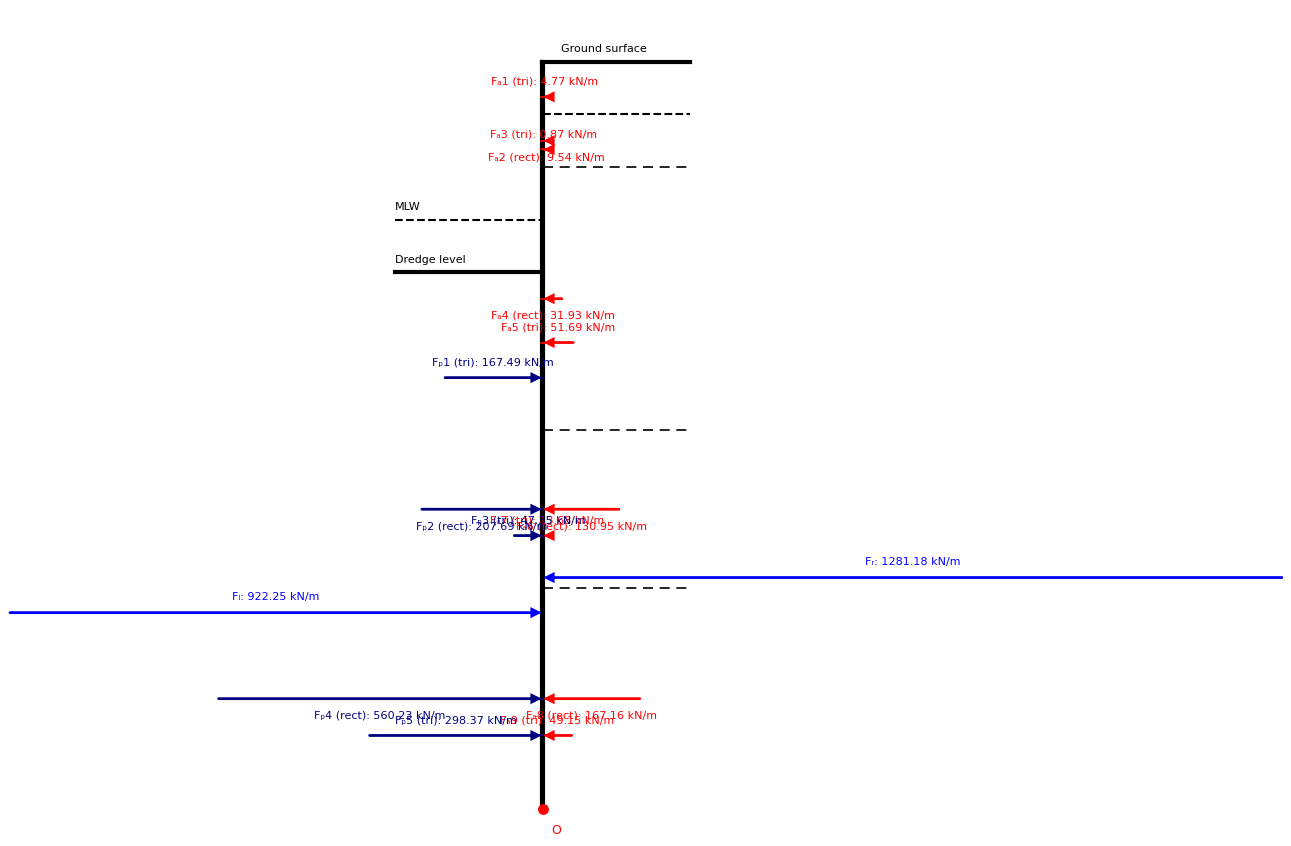
\includegraphics[width=0.90\linewidth]{figures/ch8/uls_combination_scale.png}
    \caption{ULS combination forces for $t = 10.196$ meters}
    \label{fig:appendix_uls_moments_balance_forces}
\end{figure}

\begin{table}[H]
  \centering
  \caption{Resultant forces, arms, and moments for $t = 10.196$ meters}
  \label{tab:appendix_forces_arms_moments_new}
  \small
  \setlength{\tabcolsep}{6pt}
  \renewcommand{\arraystretch}{1.15}
  \begin{tabular}{@{}l l r r r r@{}}
    \toprule
    Side & Shape &
    F [kN/m] & $z_{base}$ [m] &
    $M_{\text{base}}$ [kN$\cdot$m/m] \\
    \midrule
    ACTIVE & Triangle  &   4.77  & 13.53 &   64.52 \\
    ACTIVE & Rectangle &   9.54  & 12.70 &  121.10 \\
    ACTIVE & Triangle  &   0.87  & 12.53 &   10.91 \\
    ACTIVE & Rectangle &  31.93  &  9.70 &  309.57 \\
    ACTIVE & Triangle  &  51.59  &  8.86 &  458.14 \\
    ACTIVE & Rectangle & 130.95  &  5.70 &  745.87 \\
    ACTIVE & Triangle  &  13.68  &  5.20 &   71.11 \\
    ACTIVE & Rectangle & 167.16  &  2.10 &  350.69 \\
    ACTIVE & Triangle  &  49.15  &  1.40 &   68.74 \\
    HYDRO PASSIVE & Triangle  & 922.25 &  3.73 & -3441.82 \\
    HYDRO ACTIVE & Triangle  & 1281.18 & 4.40 & 5635.44 \\
    PASSIVE & Triangle  & 167.49  &  8.20 & -1372.72 \\
    PASSIVE & Rectangle & 207.69  &  5.70 & -1182.97 \\
    PASSIVE & Triangle  &  47.35  &  5.20 &  -246.00 \\
    PASSIVE & Rectangle & 560.23  &  2.10 & -1175.33 \\
    PASSIVE & Triangle  & 298.37  &  1.40 &  -417.31 \\
    \midrule
    $\sum M_{t}$ (should ≈ 0 for equilibrium) & & & & -0.0763 \\
    \bottomrule
  \end{tabular}
\end{table}

\begin{figure}[H]
    \centering
    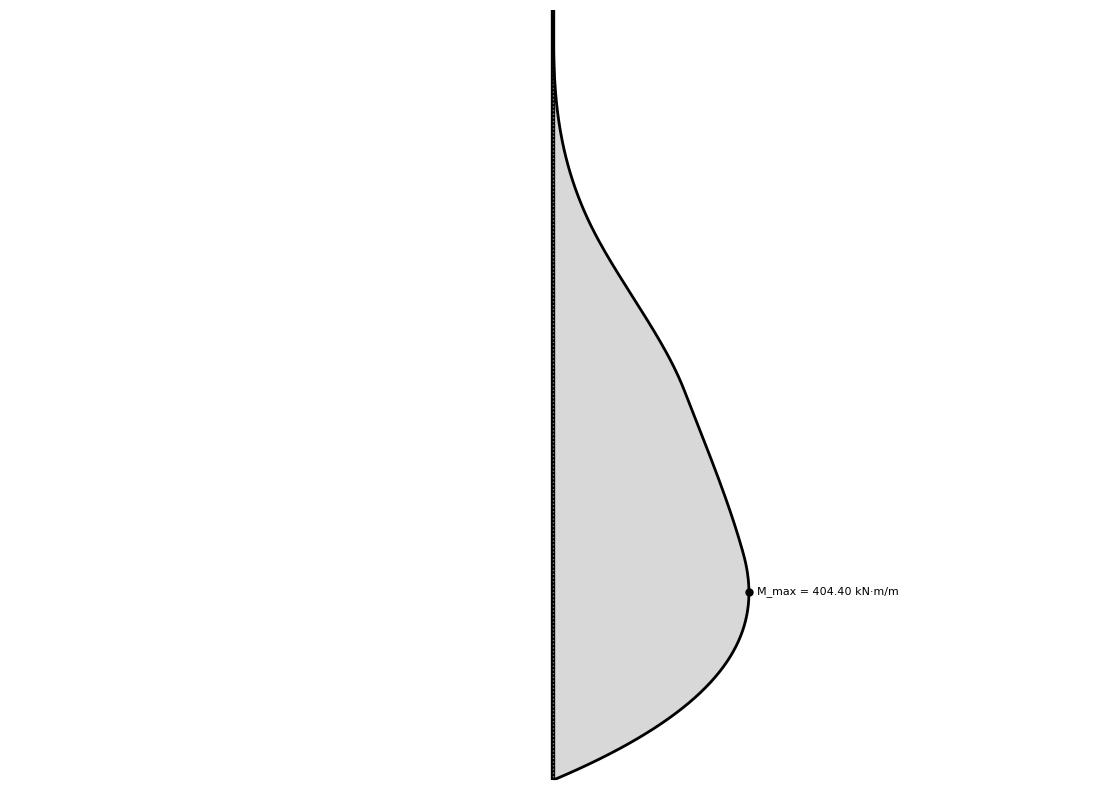
\includegraphics[width=0.80\linewidth]{figures/appendix-i/bending_moments_line_DA1_2.png}
    \caption{Bending moment line DA1-2}
    \label{fig:appendix_bending_moments_DA1_2}
\end{figure}

\begin{table}[H]
  \centering
  \caption{Moment calculation summary DA1-2}
  \label{tab:moment_summary_DA1_2}
  \small
  \setlength{\tabcolsep}{8pt}
  \renewcommand{\arraystretch}{1.15}
  \begin{tabular}{@{}l r@{}}
    \toprule
    Quantity & Value \\
    \midrule
    Depth below ground [m] & 10.721 \\
    Depth below dredge [m] & 6.721 \\
    $M_{a,\text{soil}}(S)$ [kN·m/m] & 922.641 \\
    $M_{wR}(S)$ [kN·m/m] & 1294.480 \\
    $M_{a}(S) = M_{a,\text{soil}} + M_{wR}$ [kN·m/m] & 2217.121 \\
    $M_{p,\text{soil}}(S)$ [kN·m/m] & 857.051 \\
    $M_{wL}(S)$ [kN·m/m] & 955.664 \\
    $M_{p}(S) = M_{p,\text{soil}} + M_{wL}$ [kN·m/m] & 1812.715 \\
    $M_{\text{max}} = M_{a}(S) - M_{p}(S)$ [kN·m/m] & 404.406 \\
    \bottomrule
  \end{tabular}
\end{table}

\begin{figure}[H]
    \centering
    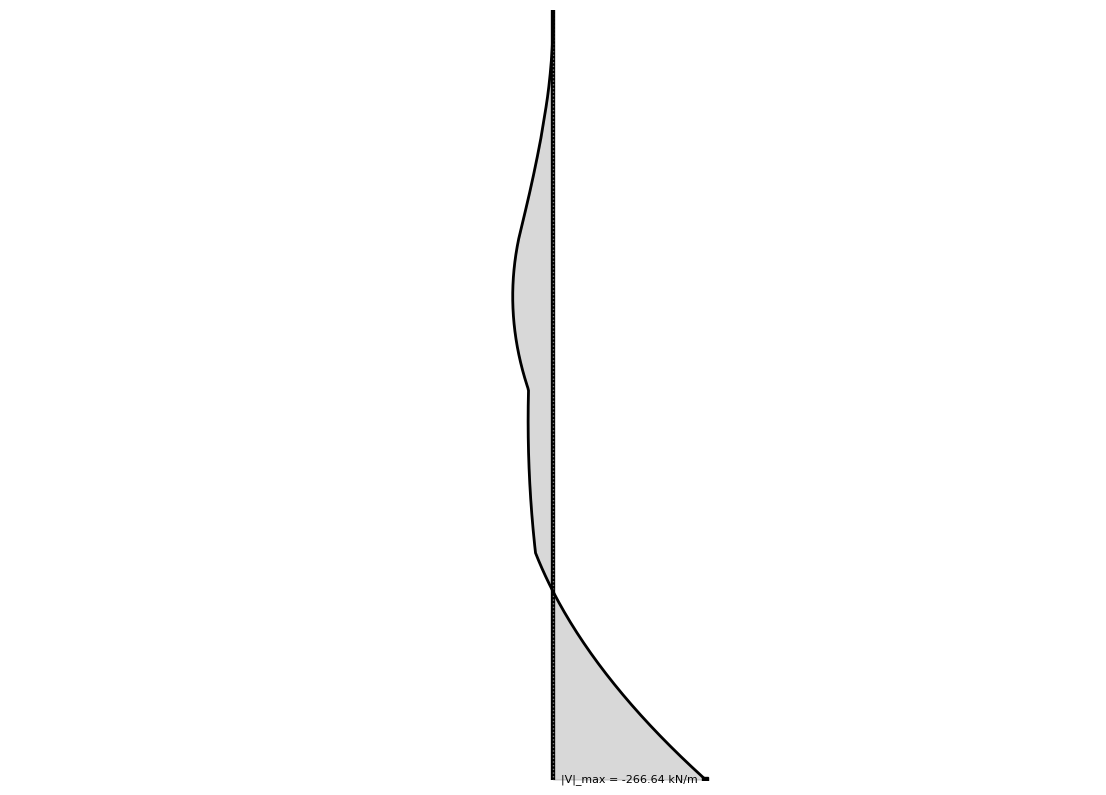
\includegraphics[width=0.80\linewidth]{figures/appendix-i/shear_max_10172.png}
    \caption{Shear force line DA1-2}
    \label{fig:appendix_shear_forces_DA1_2}
\end{figure}

\begin{table}[H]
  \centering
  \caption{Shear and partial-resultants summary}
  \label{tab:shear_summary_zs_caseB}
  \small
  \setlength{\tabcolsep}{10pt}
  \renewcommand{\arraystretch}{1.15}
  \begin{tabular}{@{}l r@{}}
    \toprule
    Quantity & Value \\
    \midrule
    Zero-shear depth $z_S$ [m] & 10.721 \\
    Depth below dredge at $z_S$ [m] & 6.721 \\
    $V(0)$ at ground [kN/m] & 0.000 \\
    $V(Z)$ at dredge [kN/m] & 55.882 \\
    $V(z_S)$ [kN/m] & 0.000 \\
    $V(z_{\text{toe}})$ [kN/m] & -266.635 \\
    $|V|_{\max}$ [kN/m] & -266.635 \\
    Depth of $|V|_{\max}$ [m] & 14.172 \\
    $V_a(0\to z_S)$ [kN/m] & 257.468 \\
    $V_{wR}(\text{wt}\to z_S)$ [kN/m] & 419.782 \\
    $V_p(Z\to z_S)$ [kN/m] & 334.353 \\
    $V_{wL}(\text{wl}\to z_S)$ [kN/m] & 342.897 \\
    Left-to-right sum @ $z_S$ [kN/m] & 0.000 \\
    \bottomrule
  \end{tabular}
\end{table}





